\chapter{最短路径优化算法研究综述}

\section{图}

\subsection{图的基本概念}
图论,是组合数学分支,和其他数学分支也有密切关系,如群论、拓扑学。图是图论的主要研究对象,图是给点若干顶点以及两顶点所构成的图形,这种图形可以用来描述事物之间的某种特定关系。
顶点可以用来描述某种事物,连接两顶点可以代表事物之间存在的某种关系,如顶点代表学习任务,连接顶点代表学习该任务之前需要学习的其他任务。图论起源于著名的柯尼斯堡七桥问题即著名的欧拉图一笔画问题。该问题于1736年被欧拉解决,因此普遍认为欧拉是图论的创始人\cite{r1}。通常在图论中,以有序对$G=(V,E)$,其中V是点集;$E\subset \{\{x, y\}:(x,y)\in V^2,x\ne y\}$是边集,由所有顶点序列构成,其中一条边$\{x,y\}$中的x,y被称作边的端点;
图的分类分为有向图和无向图,其中有向图是指给图的每条边都规定一个方向,其边称为有向边,以$<x,y>$;相反,边没有方向的图称为无向图,无向边以$(x,y)$表示,则在边集会同时存在$(x,y),(y,x)$。并且V,E的元素个数通常都是有限的,图的阶数是其顶点个数$|V|$,图的边数是$|E|$。每条边都连接两个不同的顶点且没有两条不同的边连接一对相同顶点的图称为\textbf{简单图},可能有\textbf{多重边}连接同一对顶点的图成为\textbf{多重图}。其中最短路径问题、最小生成树问题、关键路径问题都属于是基于图上的问题,并提出了相应的解决方案。如图\ref{fig:graph_ex}分别是无向图和有向图的一个实例。其中,对于实际问题中每条边代表了从顶点$x$到$y$所需要的权值的图叫做带权图,其中边上的权值也叫边的长度。
\begin{figure}[htbp]
  \centering
  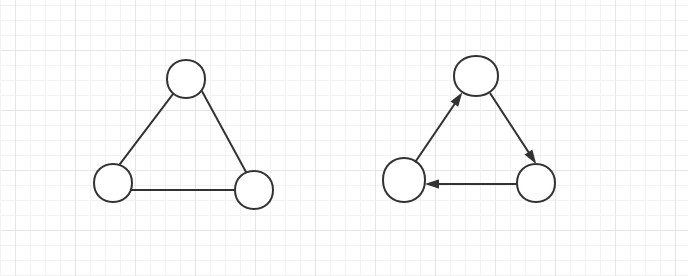
\includegraphics[width=10cm]{figures/graph_ex.png}
  \caption{无向图和有向图实例}  
  \label{fig:graph_ex}
\end{figure}
\par\textbf{三维空间}是类似我们生存的空间的数学模型,由长、宽、高三个维度,也即是三维欧几里得空间,定义欧几里得平面为装备了内积的二维实数的向量空间。满足
\begin{enumerate}[.]
    \item 在这个向量空间中的向量对应欧几里得平面中的点,
    \item 在向量空间中的加法运算对应于平移,
    \item 内积蕴含了角和距离的概念,它可被用来定义旋转。
\end{enumerate}\par
如图\ref{fig:3axis}就是三维欧几里得空间的示意图,三个轴相互垂直,点的坐标为其到三个轴的投影。
\begin{figure}[htbp]
  \centering
  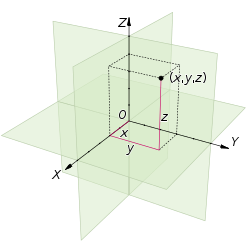
\includegraphics[width=8cm]{figures/3axis.png}
  \caption{三维欧几里得空间}  
  \label{fig:3axis}
\end{figure}
\subsection{图的存储表示}
一般在计算机中存储图信息,有以下几种方式
\begin{enumerate}
    \item 邻接矩阵,使用多维数组记录点与点之间的边权信息;
    \item 邻接表,使用链表等数据结构维护该点到其他点的边信息;
    \item 十字链表,将有向图的邻接表和逆邻接表的结合;
    \item 邻接多重表,将无向图的邻接表和逆邻接表的结合;
\end{enumerate}\par
邻接矩阵是应用多维数组保存的点和点之间的关系,因此可以很容易的判断两个点之间的关系,但缺点在于占用空间大,尤其对于多维空间时保存信息时需要占用大量的存储空间;邻接表使用链表保存点所连接的边信息,节省了空间,但不易得到两点之间的关系;十字链表和邻接多重表都能节省空间、快速判断点与点之间的关系,但缺点是实现起来比较复杂。

\section{路径规划}
首先,在图中的\textbf{路径}是指从顶点$u$到顶点$v$的一个序列$v_0,e_1,v_1,e_2,v_2,\dots,e_k,v_k$,有时简写为$v_0\rightarrow v_1\rightarrow v_2\rightarrow\dots\rightarrow v_k$,其中$e_i$表示起点终点为$v_{i-1}$及$v_i$;$k$称为路径的长度,即经过的边的数量;$v_0=u$称为路径的起点;$v_k=v$称为路径的终点。当没有必要区分多重边时,就用顶点序列$x_0,x_1,\dots, x_n$表示通路$e_1,e_2,\dots,e_n$,其中对于$i=1,2,\dots,n,f(e_i)={x_{i-1}, x_i}$,这种记法仅仅指出通路所经过的顶点。其中论文求解的最短路径是指:若从顶点$u$到顶点$v$之间长度最短的路径,即是加权图中一条路径的长度是这条路径上各条边的总和最小。
\section{最短路径规划算法}
最短路径问题是图论研究的一个经典算法问题,目的在于求出两顶点之间的最短路径。算法具体的形式有
\begin{itemize}
    \item 确定起点的最短路径问题,也即已知起始起点求最短路径的单源最短路径问题;
    \item 确定终点的最短路径问题,与确定起点的问题相反,该问题是已知终结顶点,求最短路径的问题;
    \item 确定起点终点的最短路问题,即已知起点和终点,求两顶点之间的最短路径;
    \item 全局最短路径问题,也叫多源最短路问题,求出图中所有的最短路径。
\end{itemize}
\par 用于解决最短路径问题的算法叫做“最短路径算法”,常用的路径算法有:
\begin{itemize}
    \item BFS算法;
    \item Dijkstra算法;
    \item A*算法;
    \item Bellman-Ford算法;
    \item SPFA算法(Bellman-Ford算法的改进版本);
    \item Floyd算法;
\end{itemize}
\par 广度优先搜索(BFS)和深度优先搜索(DFS)会从起点开始求解出可行路径,但由于DFS需要求解所有路径才知道最短路径,而BFS算法的特点是逐层扩展的,决定了其不需要遍历所有的路径就能找到最短路径。Dijkstra、A*、Bellman-Ford、SPFA算法都是用于解决单源最短路径,其中Dijskra用于正权路径最短路径求解,Bellman-Ford、SPFA、A*可用于正负权路径最短路径求解,Floyd用于解决多源最短路径;其中不同算法在基于不同的图结构上拥有不同的时间、空间复杂度,其中Dijkstra和A*在寻路算法中应用广泛,由于A*使用了估值函数,会更倾向的选择路线,更加节省内存空间。
\section{本章小结}
\par{\kaishu 本章主要介绍了图结构的定义以及常见的计算机存储图结构的数据结构,以及介绍了路径定义和最短路径的定义和求解算法。对于常见的图结构,使用邻接矩阵和邻接表在不同的应用领域都有很好的发挥,如邻接矩阵可以很快的得到顶点与顶点之间的关系,但需要记录每个顶点到其他所有顶点的关系,占用的内存空间较大;邻接表使用链表结构存储每个顶点所连接的边信息,可以节省大量的空间,但不容易得到顶点与顶点的关系。随后介绍了关于对图上最短路径求解的常用算法,如单源最短路径算法,有用于正权图最短路径求解的Dijskra算法,正负权都适用的Bellman-Ford、SPFA算法,基于估值函数优化的A*算法在寻路方面有广泛的应用;以及用于多源最短路径求解的Floyd算法。}